
\renewcommand*{\thesection}{\Roman{section}.}
\renewcommand*{\thesubsection}{\arabic{section}.\arabic{subsection}}

\chapter*{Introduction}
\markboth{\bf INTRODUCTION}{}

Advances in biochemistry and molecular genetics have been concerned with gene action, protein synthesis, and protein structure. Thus we now have a fairly detailed picture of how protein structures are determined, both as regards specific configuration and as regards the mechanism and energetics of their syntheses. Furthermore by a combination of genetic and biochemical investigations in the area usually described as `metabolism' we are obtaining an ever widening picture of the relationships between metabolic steps, often displayed as metabolic maps which show in a qualitative way the flow of synthetic and degradative pathways (anabolism and catabolism). Although this picture is by no means complete there is a general feeling that the major structure of living systems, at this level, is known. Broadly speaking the genetic specification, i.e. the base sequence of the DNA, determines the parameters (quantity, turnover numbers and Michaelis constants) of the enzymes which catalyse the biochemical transformations of the metabolic network. What is much less understood, however, is how such specifications affect the quantitative outcome of the multiple interactions within a metabolic system which, in the end, determines the measurable properties of the whole system or organism. What is, therefore, required is a "quantitative biochemistry" as well as the relation of this to quantitative genetics, whose approach has been both historically and methodologically quite different from molecular genetics. This thesis is an attempt to relate the three fields of molecular genetics, metabolic biochemistry and quantitative genetics.

\section{Non-quantitative nature of present system theory}

During the past few decades the joint application of genetics and biochemistry to relatively simple organisms such as viruses, bacteria and syncytia has led to an increasing elucidation of their details. There has been great success in discovering system components, isolating them from homogenates, studying their properties in vitro and defining their relationship to the complete system. We now possess a fairly universal classification of system components into such types as genes, messenger RNA, ribosomes, proteins and a knowledge of their respective functions within the cell. The detailed action of these subunits may vary across strains and species but at least at the level of cell biology the general picture is fairly clear. For some types of organism such as E.coli, yeast and Neurospora a great deal is already known. Thus it is claimed that about $40 \%$ of all metabolic activity has been accounted for in {\em E. coli} K12 (J.D. Watson, 1965).

It seems then that, as this detail is added to, we shall, at the level of cell biology, be increasingly in the situation of, viewing the organism in terms of a sort of chemical engineer's block diagram. The engineer's blocks now represent the separate genetically specified transformational activities (enzyme catalysis) taking place in metabolism and the engineer's system variables become the various chemical concentrations being transformed one to another in the cell. Indeed, the cell has been viewed in just this way for a long time, the great achievement being to define and characterise what all the separate `blocks' are. Thus a large class of data is explained for a given cell type by a transformational block diagram, tentatively proposed for that cell. Such data is essentially qualitative such as, for example, whether a given enzymic activity is present or absent in the extract of a mutant or whether the mutant can grow or not on a minimal medium with a certain supplement. The block diagram explains the data insofar as it allows qualitative prediction of the effects. of hypothesised large changes to blocks within the diagram.

Thus we have a reasonably well established `qualitative system theory' of cell metabolism which is consistent with a large body of qualitative date and this theory is similar in general outline over a wide range of cell types.

More recently there has been considerable interest in extending transformational diagrams by adding to them a `control level' showing which system variables have a strong effect on the rate of any given transformation, although in this case the details have been found to vary considerably over different cell types. These studies have involved the consideration of a less qualitative type of data, for example, the measurement of low, intermediate and high levels of an enzyme in extracts of cells grown under various conditions. Nevertheless, even with the inclusion of a control level, the present system theory of cell metabolism has remained essentially qualitative in nature. Unlike the engineer, the biologist is not at present easily able to use his block diagram to predict the quantitative effects of substituting a slightly altered form of one of his blocks (enzymes) or of altering the level of an external metabolite.

What will be the form of a quantitative theory? Clearly with the existing system theory one worked from a block diagram, itself constituting the theory, and used a form of logical argument to predict the consequences of any particular lesion. With a quantitative approach it will be necessary to attach to each block in the diagram a formula of some sort giving the rate of its transformational activity. This formula being in terms of the system variables which strongly affect the block and of the genetically specified parameters which describe it.

Although any change in a block or environmental parameter will directly affect the rates of only a few activities these will affect system variables which will affect other activities and so on. The quantitative response of any system property is thus the result of a complex balance between the various activities underlying the system. In a quantitative theory prediction will thus require a calculation which allows fully for the detailed behaviour of the separate blocks as well as for the block diagram which was sufficient for a qualitative theory.

Just as the qualitative system theory aimed to explain a wide range of qualitative data, so any quantitative extension must now include a much larger body of quantitative data which, although it may not conflict with the transformational and control diagram, is by no means explained by it.

\section{Some quantitative approaches}

I shall consider first some studies which have avoided explanation of particular data and have asked instead what general properties may arise out of commonly occurring metabolic mechanisms. Thus Goodwin (1963) focussed attention on possible dynamic consequences of the feedback loops found to control enzyme quantity in a variety of cells, conjecturing that they may be in a state of spontaneous oscillation. He has further considered cellular dynamics from the point of view of there being a number of such oscillators, weakly coupled, within each cell and treated this by the methods of statistical mechanics.

Following on this and also because of the clear experimental findings concerning metabolic oscillation there has been considerable discussion of the conditions under which such oscillations could occur. J.S. Griffiths (1968a, 1968b) has considered oscillators of the Goodwin type and defined more clearly the necessary conditions, his work suggesting that rather special assumptions are required. The problem of stability has also been considered by C. Walter (1968a, 1968b). A more abstract treatment is offered by S.A. Kauffman (1969) who has considered the cell as a system in which genes have only two states, on and off, the state of a gene in the next instant of time being determined by the state of a small number of genes controlling it at the previous instant. This abstraction of a problem, not unlike Goodwin's coupled oscillators, has enabled him to consider large networks with extensive coupling and to demonstrate that a number of interesting properties are possessed by such systems. Thus it appears that a network of `genes' connected at random and with randomly assigned boolean response function to their inputs will for the case where each gene has two inputs, almost always possess only a few distinct cycles of activity into which it rapidly falls when released from an arbitrary initial condition. Furthermore these cycles of activity are surprisingly short, involving often only a very few `states' of the system before repeating. This simple cyclic or even steady state behaviour is of some interest arising as it does in systems which at first sight might be expected to generate extremely complex dynamical behaviour. A further value of Kauffman's approach is that he relates cell metabolic theory to the already much studied theory of `finite automata'.

These approaches are, however, highly abstracted formulations remote from quantitatively ascertainable data and are, therefore, not suitable to make the link between the areas with which this thesis is concerned. More relevant to our purposes are the classical biochemical approaches as follows.

\section{Enzyme kinetics}

Here there exists an extensive literature, see for example "The Enzymes" (1959), the bulk of which is concerned with studies, both theoretical and experimental, on single enzymes. The basis of these studies is usually that the enzyme can exist as a number of alternative `complexes' with its substrates, products and inhibitors and that interconversion between these is governed by the usual chemical law of mass-action.

This gives rise to a set of 1'st order differential equations involving a number of hypothetical enzymic intermediates and the necessary rate constants to describe their mass-action interconversions. The data to which this theory is related is largely derived from {\em in vitro} studies, preferably with purified enzymes, and consists of the concentrations of substrates, products, and other substances at various times after the introduction of the enzyme. Only rarely is the concentration of an enzymic intermediate monitored directly and again the early rapid reaction phase is not normally observed. Consequently for most metabolic enzymes complicated kinetic schemes should be viewed with suspicion as also their rate constants, particularly when one considers that the conditions in vivo may be very different from that of the purified enzyme in isolation.

\section{Steady state enzyme kinetics}

This considers the situation when substrates and products are held at a steady concentration and asks what is their respective rate of removal or production by the enzyme. Bimolecular reactions are usually considered to take place only between enzymic intermediates and metabolites, protein interactions not normally being included. Under these circumstances a set of simultaneous equations can be written down which define the steady state levels of the various enzymic complexes and since these equations are linear in terms of the enzyme complexes it is possible to solve them explicitly. This yields the overall `rate' of the reaction as an algebraic expression involving the steady levels of the metabolites and the various rate constants characteristic of the protein. King and Altman (1956) have provided an elegant method for writing down the `rate expression' directly from a diagram of the kinetic scheme. The results of applying this systematically to a variety of kinetic schemes has been presented by W.W. Cleland (1963) who also advocates that the expressions be written using Michaelis constants and other enzyme kinetic constants which can be defined operationally, rather than with elementary rate constants. The simplest expression appearing in Cleland's paper being for the well known case of an enzyme catalysed reaction having one substrate and one product (H.L. Segal, 1959), when the rate expression takes the form
%
$$
\mathrm{FLUX}=\frac{\mathrm{ET} / M\left(S_{1}-S_{2} / K_{E}\right)}{1+S_{1} / M+S_{2} / M}.
$$
%
where $E$ is the concentration of the enzyme.

Here $M, M$ are Michaelis constants which are usually obtained directly from an assay for the forward and reverse reactions respectively as could $T$ the turnover number corresponding to `maximum velocity' in the forward direction. $K_{E}$ is the equilibrium constant for the reaction $S_{1} \rightarrow S_{2}$ This equation reduces to the well known rate expression due to Briggs \& Haldane (1925) when $S_{2}$ is set at zero.

This flux is a good approximation to the instantaneous value, even when the pools are varying slowly (Richards and Pring, 1968). We shall make use of equations of this type in later chapters. The rate expressions for even slightly more complicated kinetic schemes can become very cumbersome. Consequently several workers, for example R.O. Harst (1968) have resorted to programming the King Altmann method so that these more complicated rate equations can be produced automatically on a digital computer from a description of their kinetic schemes.

\section{Multi-Enzyme systems}

Perhaps the most consistent attempt at a quantitative treatment of a specific multi-enzyme system has been in relation to the glycolytic pathway, started by Chance in 1951. Since that time B. Chance, D.Garfinkel, J. Higgins and other workers have continued to develop experimental, theoretical and computer techniques - recently reviewed by D. Garfinkel (1970). Their reason for becoming involved in computer techniques is that the mathematical representation of even a simplified multi-enzyme system involves a large number of non-linear differential equations which cannot be handled by existing analytic techniques and have consequently to be solved by `simulation' on a digital or analogue computer. Their main interest has been in a study of the transient effects in the glycolytic pathway based on work with mouse ascites cells (B. Chance et al., 1960) and with heart and liver, (Garfinkel et al. 1968).

Long computation times are found in these systems, mainly due to the commonly encountered situation that the molar concentration of enzymic intermediates is much lower than that of metabolic intermediates. This produces high frequency components in the D.E. and the step length of the numerical integration procedure used has to be sufficiently small to cope with these. As a result considerable amounts of computer time can easily be expended in representing only a little `real' time in the biochemical system (Garfinkel, 1965).

Consequently an effort has been made to improve the methods of integration employed in simulation programmes so that they are more suitable for handling the `stiff' equations commonly encountered (Cooper, 1970). Recently (Curtis, A., unpublished data, 1970) the predictor-corrector method of Gear (1968) has been employed on a simulation problem, previously run using the method of E. Chance (1969), with a claimed improvement in speed of 100 times.

Another approach to the problem of computer efficiency has been to use the rate-equations of steady state enzyme kinetics which were discussed earlier, thus removing the differential equations corresponding to enzymic intermediates, which are mainly responsible for the stiffness encountered in biochemical systems. These rate equation representations are now, of course, only an approximation to the `true' dynamics but this will not normally be a serious discrepancy (Rhoads and Pring, 1968).

A problem which has received considerable attention is that of how to `describe' the biochemical system to the computer and the more recent programs of Gerfinkel (1968) and of E. Chance (1969) will accept a form of biochemical-language which is meaningful to the experimental biochemist. For programmes employing mainly rate-equation methods the use of a biochemical language is not so straightforward but, (Rhoads and Pring, 1968), methods have been devised to generita these automatically and link them into the commonly employed simulator programs (Garfínkel, 1968).

Some unexpected results have arisen on the experimental side. Thus Chance et al. (1964) find sustained oscillations, apparently arising at the level of intermediary metabolism. This has stimulated theorist's, as for example Achs and Garfinkel (1968) to construct oscillatory models. Again Garfinkel (1969) remarks that very few enzymes, working in situ, behave as they do in isolation.

All of the quantitative work just mentioned assumes implicitly that the cell can be regarded as chemically homogeneous or `well mixed', although it is possible to include a limited type of inhomogeneity.

\section{The problem}

The purpose of this thesis is to develop a suitable theoretical framework together with relevant computer techniques, which it is hoped will illuminate the beheviour of genetical systems. By genetical systems is meant an organism (or its analogue) or a population of organisms which is specified by a set of initial parameters (genes and environment) and into which we can introduce variation. Such variation will be introduced either by considering alternative functional alleles at one or more genetic loci, or by changes in the environment.

An alternative allele will be represented by a quantitative change in the specification of a catalytically active molecular species (enzyme) while the environmental variation will be represented by a quantitative change in the concentration of one or more external sources of metabolites.

The essence of genetic methodology is the measurement of difference between organisms or populations. Which measurements are taken is arbitrary, but an analysis of systemic behaviour requires that the functional dependence of any measure is analysed in terms of the effect of the imposed variation on the system. our task, therefore, is to investigate how a metabolically organised system responds to variation in the parameters. which define it.

The measures in which we are interested are mainly time independent averages of some sort and are usually of a biochemical nature. Some examples would be concentration of a metabolite, quantity of an enzyme in a cell, net-flux in a metabolic pathway. The averages being obtained by sampling from a large exponential growing population, of asynchronous cells, from a single syncytium in exponential growth or from particular tissues of adult metazoa. Consequently we can argue (Chapter I) that a suitably extended `steady state' treatment of metabolism is the appropriate development from qualitative system theory. This steady state treatment must, however, include bimolecularity, inhibition of enzyme activity, repression and induction of enzyme quantity, saturation properties of enzymic reactions, and networks of arbitrary complexity since these are essential aspects of any real system and cannot be ignored without sacrificing important features of quantitative behaviour. It should be stressed that although much has been written on the theory of the steady state this literature has dealt almost exclusively with `linear' systems leaving out of consideration the non-linear phenomena mentioned above.

\begin{figure}
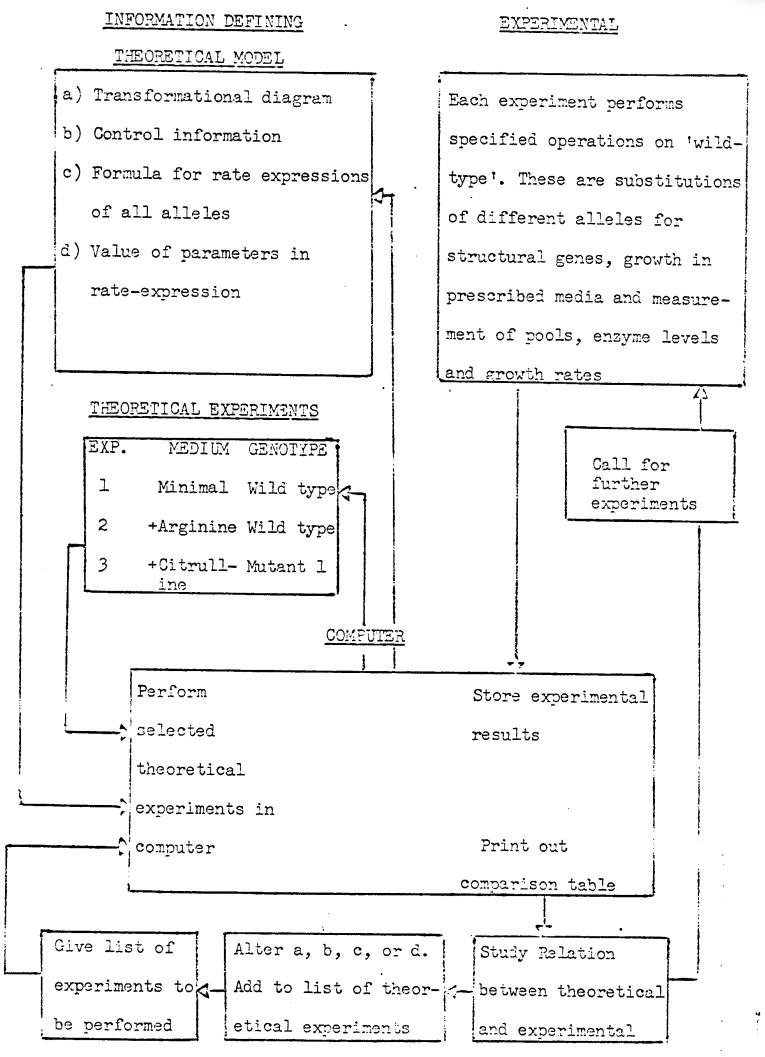
\includegraphics[scale = 1]{figure0_1.png}
\end{figure}

\section{Role of computer in relation to quantitative experiments}

Let us consider how one would set about establishing such a quantitative model within an area of metabolism where the block structure and the control structure has been tentatively established by means of qualitative information.

I have in mind particularly the sort of work which is being carried out in laboratories studying pathways in structurally simple organisms, but it is by no means restricted to these. Essentially the procedure is to measure a number of system variables, metabolic pools, enzyme levels, flux in pathway, both for the wild type organism and for strains with various quantitatively altered forms of enzymes. These `quantitative' mutants may be obtained as revertants from known mutants, affecting structural loci, which abolished enzyme activity, or may be discovered as natural variants. Measurements are taken both on minimal medium and on medium containing various supplements.

Thus a fairly large amount of data is gathered to which the proposed quantitative model must conform. In addition there will be some rough information, gained from in vitro studies, atout rate expressions for the wild type and mutant enzymes which will be helpful in formulating the initial theoretical model. Similarly, this kind of information may become available from natural or domestic animal populations. The facing diagram indicates an example of the necessary procedure.

There are several interesting features of this process which should be noted. Firstly, it can be seen that the computer plays an essential role. Without it the theoretical model could not be evaluated against the facts. Secondly, the process is not to be thought of as simply adjusting the parameters of a fixed model to fit the data by, for instance, hill climbing on some least squares procedure. Rather the process is more `scientific' than `statistical'. Thus not only the parameters but also the block diagram, the assumptions about control or the form of the rate expressions are all subject to alteration as the model is studied in relation to data.

A good example of this scientific situation and of the integral role of the computer is that the computer can be used to decide a quantitative question that of ten arises. Which of several experiments is likely to discriminate most sharply between currently competing hypotheses about the model?

Thirdly, it seems that the building up of a quantitative model is a more interactive process than was that for the qualitative model. Thus when we adjust our assumption about one part of the model to meet some new experiments we may disturb existing agreement with previous experiments. The computer is again invaluable here as it enables us to retest agreement with all previous experiments every time we adjust the model.

If this process of interaction between biological data and computer model proves successful the result would be twofold:

(1) We would be in possession of a model which consistently reflects the qualitative and quantitative results of the experimental data. This means that our confidence in having the "correct" model is strengthened. (2) We would have at our disposal a predictive tool which enables us to investigate novel situations which are either difficult, lengthy, or expensive to perform on biological material. This process is usually described as `simulation' and forms the goal of many investigations (and has been successfully applied in many fields of engineering). In the next section we shall argue, however, that this may fail on grounds of feasibility and, more importantly, that the general properties of quantitative systems may be used to answer questions of theoretical importance beyond the problem of the simulation of a particular organism (Kacser and Burns, 1968).

\section{General strategy for quantitative approach.}

At this point we must take stock of the general position in which quantitative cell metabolism is at the moment.

Firstly, if the aim is the setting up of an exact-quantitative model of metabolism in some cell type, we must first argue the value of having such a model. Often the effort required to establish the model will be out of all proportion to its value. Secondly, the feasibility of setting up a \underline{comprehensive} model of metabolism is doubtful at the present time, even for E.\ coli and certainly for all other cell types. Thus in most cases not even the necessary qualitative knowledge has been obtained. A more fundamental reason, however, is for instance, that the form of the rate expression of many enzymes, even in vitro, is still controversial and appears likely to remain so.

The strategy advocated here is that we should concentrate on acquiring the ability to incorporate quantitative information into a predominantly qualitative picture, and not to worry too much about details. As the need and opportunity arises this ability can be applied to various situations. Clearly just as the block diagram has been gradually extended over a period of many years so a qualitative model can gradually be turned into a quantitative model as the necessary reliable data on system disturbance and system response becomes available.

\section{Theoretical treatment of metabolic systems}

We have above painted a rather gloomy picture of the immediate prospects for a comprehensive quantitative approach based on real data and have also questioned its general usefulness, whilst pointing out the relation of computational and theoretical techniques to it.

However the same techniques can, just as easily, be applied to the construction and investigation, either by analysis or numerical exploration, of abstract metabolic systems expressed in the form of mathematical models. These abstract systems being chosen to posses structure, mechanisms and parametric values which are broadly similar to those of real systems. Many features of the quantitative response of real systems to parametric variation are not critically dependant on the exact parametric values obtaining. Such features, including the common occurrence of intra and inter locus interaction, the remarkable buffering ability against parametric change (Kacser, 1963) and so on, clearly arise mainly from the overall structure of the system rather than its precise parametric values. Accordingly we shall argue that it is legitimate to study such quantitative features, of systemic response to parametric variation, for suitably chosen abstract systems per se and this is in fact a major aspect of the thesis.

In principle this can be done by the numerical investigation of a wide variety of abstract systems over a wide variety of parameter values but in practice such {\em in numero} experiments are seldom informative (A. Robertson, 1967) owing to the large number of parameters involved in even the simplest model. Because of this considerable attention has been paid, whenever possible, to the algebraic investigation of system behaviour, both in a general way and, in more detail, for simple systems such as a chain of enzymes. In these studies it has proved useful to introduce the `sensitivity coefficient' (Kacser and Burns, 1968; Burns, 1968) as an index of response and to show how these coefficients are related to the quantitative behaviour of the individual parts of a system. The theoretical properties of these coefficients can then be used to discuss features of parametric response, such as `buffering', in a general way. A similar coefficient has been used by J. Higgins (1963) although in a somewhat different context.

Arising from such a treatment it may be possible to consider populations of biochemical systems which differ from each other in many parameters. This is the implicit assumption of quantitative genetics, but the usual theoretical method (e.g. Fraser, 1962, 1967) of handling metric characters in population problems has been to set up arbitrary genotype-phenotype relationships. A quantitative biochemical treatment, however, considerably restricts and defines the relationships insofar as `additivity', `epistasis', and `dominance' must not be postulated but will (or will not) arise from the underlying metabolic structure of the organisms. We shall consider a number of aspects in this manner for a simple abstract system and will suggest methods for investigating more complex systems by numerical means (Burns, 1970). 